% ===================================================================
% OpenDriveFM -- CVPR submission
%
% Replaces opendrivefm_paper.tex, which describes the retired project
% and whose numbers do not reproduce. Nothing from that file is reused.
%
% When the official template for the target year is released, drop
% cvpr.sty beside this file; the preamble picks it up automatically and
% the fallback geometry below is ignored.
%
%   latexmk -pdf main.tex
% ===================================================================
\documentclass[10pt,twocolumn,letterpaper]{article}

\IfFileExists{cvpr.sty}{%
  \usepackage[review]{cvpr}%
}{%
  % Fallback that approximates the CVPR measure closely enough to judge
  % length and figure fit. NOT camera-ready. Swap in cvpr.sty.
  \usepackage[margin=0.75in,top=1in,bottom=1in]{geometry}%
  \setlength{\columnsep}{0.3125in}%
}

\usepackage{times}
\usepackage{graphicx}
\usepackage{amsmath,amssymb}
\usepackage{booktabs}
\usepackage[table]{xcolor}
\usepackage{array}
\usepackage{colortbl}
\usepackage{microtype}

\definecolor{odfmlink}{rgb}{0.07,0.41,0.66}
\usepackage[pagebackref,breaklinks,colorlinks]{hyperref}
\hypersetup{linkcolor=odfmlink,citecolor=odfmlink,urlcolor=odfmlink}
\usepackage[capitalize]{cleveref}

\graphicspath{{../outputs/figures/}}

% Every number below that appears in prose also appears in a JSON
% artifact under outputs/artifacts/. Macros so a corrected measurement
% is a one-line change rather than a grep.
\newcommand{\Hii}{+0.0484}
\newcommand{\HiiCI}{[+0.0390,\,+0.0584]}
\newcommand{\objObs}{0.7623}
\newcommand{\objMSP}{0.7193}
\newcommand{\objDelta}{+0.0432}
\newcommand{\objDeltaCI}{[+0.0135,\,+0.0708]}
\newcommand{\objOracle}{0.7745}
\newcommand{\voxMSP}{0.8797}
\newcommand{\voxObs}{0.6321}
\newcommand{\frmConf}{0.8618}
\newcommand{\frmObs}{0.8066}
\newcommand{\missHi}{47.3\%}
\newcommand{\missLo}{4.7\%}
\newcommand{\nObj}{40{,}863}
\newcommand{\nFrames}{6{,}016}
\newcommand{\nScenes}{75}
\newcommand{\splitdigest}{\texttt{924a44db544d4818}}
\newcommand{\fullpx}{965.0}

\def\paperID{0000}
\def\confName{CVPR}
\def\confYear{2027}

\begin{document}

\title{Confidence Cannot Flag What the Model Never Considered:\\
       Geometric Observability for Camera-Only Occupancy}

\author{%
Akila Lourdes Miriyala Francis\quad Akilan Manivannan\\
Long Island University, Brooklyn\\
{\tt\small akialourdes.miriyalafrancis@my.liu.edu}\quad
{\tt\small akilan.manivannan@my.liu.edu}
}

\date{}
\maketitle

% -------------------------------------------------------------------
\begin{abstract}
Camera-only occupancy models are evaluated almost entirely by how often
they are right, and their uncertainty is read off their own softmax. We
ask a different question: can a purely geometric quantity, computed from
the sensor rig and the ego pose and never from the network, tell us where
such a model is about to be wrong? We define \emph{observability}, a
continuous per-voxel measure of how well the camera array actually sees a
point in space, with a single parameter and no learning. On
Occ3D-nuScenes, observability ranks per-voxel error better than the
dataset's own \texttt{mask\_camera} flag by \Hii\ \HiiCI\ AUROC on a
sealed test split.
%
The result we did not expect is an inversion across granularity. Predicting
whether an individual voxel is wrong, the model's own confidence dominates
geometry by a wide margin (\voxMSP\ against \voxObs). Predicting whether a
whole \emph{object} is missed entirely, geometry wins (\objObs\ against
\objMSP, a gain of \objDelta\ \objDeltaCI\ over \nObj\ objects), and comes
within noise of a LiDAR point-count oracle (\objOracle). The mechanism is
simple and, we argue, general: confidence is a statement about a
prediction that was made, so it is near-tautologically good at flagging a
wrong one, and structurally unable to flag a prediction that was never
made at all. Where a missed object should be, the model is confidently
predicting free space.
%
All hypotheses in this paper were registered in an append-only log before
the corresponding data existed. We report the four that did not survive
alongside the ones that did.
\end{abstract}

% -------------------------------------------------------------------
\section{Introduction}

% MAD opens on animators drawing an animatic. The equivalent concrete
% opening here is the failure itself, not a literature survey.
A camera-only occupancy model asked about a volume of space it cannot see
does not abstain. It predicts free space, and it does so confidently.
Nothing in the model's output distinguishes ``there is nothing here'' from
``I have no evidence either way'', because both arrive as a high-probability
vote for the free class. On the held-out scenes used throughout this paper,
\missHi\ of annotated dynamic objects standing in volumes with no camera
evidence are not predicted by the model at all. \Cref{fig:qualitative} shows one of them.

% TODO(paper): one paragraph on why this matters downstream -- planner
% consumes occupancy as if absence of evidence were evidence of absence.

The usual answer is to calibrate the model's own confidence. We show this
answer is adequate for one question and structurally inadequate for
another, and that the boundary between them is the granularity of the
thing being asked about.

% TODO(paper): the gap, stated as a claim a reviewer could disagree with.

We therefore propose \emph{observability}, a geometric measure computed
entirely outside the network:
\begin{enumerate}\itemsep0pt
\item it is a function of the camera rig and the ego pose, so it is
      available before the model runs and is unchanged when the model
      changes;
\item it is continuous, where the dataset's \texttt{mask\_camera} flag is
      binary and, as we show, is not a visibility measure at all; and
\item it carries exactly one parameter, fixed once at \fullpx\ and never
      retuned per model or per split.
\end{enumerate}

\paragraph{Contributions.}
\begin{itemize}\itemsep0pt
\item A geometric, learning-free observability measure that ranks
      camera-only occupancy error better than the dataset's own camera
      mask by \Hii\ \HiiCI\ AUROC on a sealed test split.
\item The granularity inversion: confidence dominates geometry per voxel
      and per frame, geometry wins per object, and we give the mechanism
      that predicts this rather than observing it after the fact.
\item An evaluation protocol in which every hypothesis is registered with
      its acceptance criterion before the data exists. Four of ten
      decided hypotheses failed, and all four are reported
      (\cref{tab:ledger}).
\end{itemize}

\begin{figure}[t]
\centering
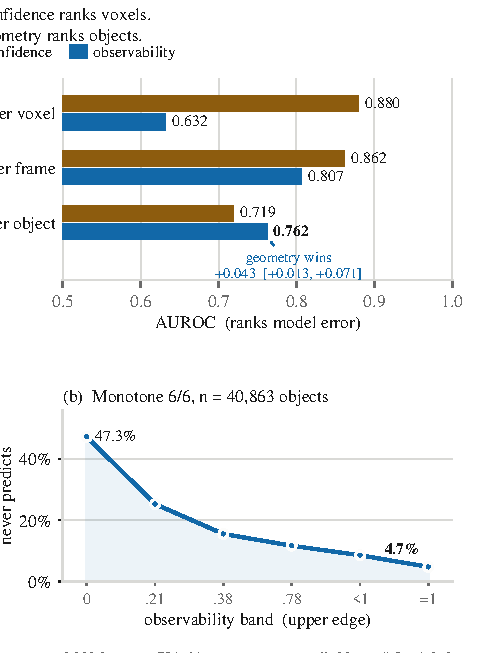
\includegraphics[width=\linewidth]{fig1_granularity.pdf}
\caption{\textbf{Confidence ranks voxels; geometry ranks objects.}
(a)~AUROC for ranking model error at three granularities on the sealed
test split. The model's own confidence dominates geometry per voxel and
per frame, then \emph{loses} per object. (b)~The mechanism: the fraction
of annotated dynamic objects the model never predicts, against
observability, monotone across all six bands over \nObj\ objects.
Confidence cannot flag what the model never considered.}
\label{fig:teaser}
\end{figure}


\begin{figure*}[t]
\centering
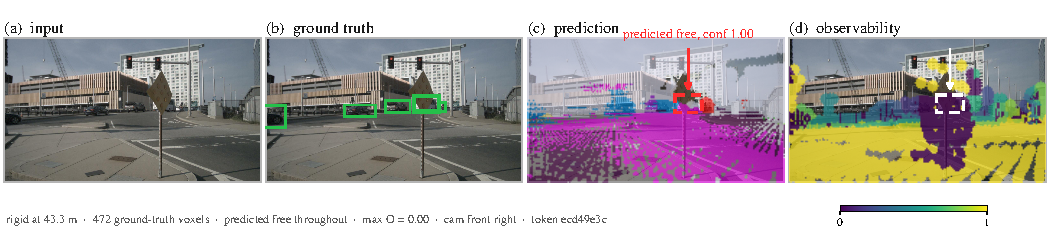
\includegraphics[width=\textwidth]{fig2_qualitative.pdf}
\caption{\textbf{One frame, and the failure this paper is about.}
(a)~The camera that should see the pedestrian: it stands behind a lamp post,
into direct sun. (b)~Occ3D ground truth, dynamic classes in red; the
pedestrian is there. (c)~The FB-OCC prediction over the same volume: nothing
inside the circle, and the model assigns the free class there at confidence
$1.00$. Its softmax offers no signal at all, because a confident prediction
of \emph{free} is exactly what a missed object looks like. (d)~Observability
for the same frame. The lamp post casts a zero-observability wedge, and the
pedestrian sits inside it, $\mathrm{obs}=0.00$. The geometry knows the
volume is unobserved before the network runs, and knows it without ever
seeing the network's output.}
\label{fig:qualitative}
\end{figure*}

% -------------------------------------------------------------------
\section{Related Work}

\subsection{Camera-only occupancy prediction}
Dense 3D occupancy has become the representation of choice for camera-only
perception because it describes arbitrary geometry rather than a fixed set
of boxes. BEVFormer~\cite{li2022bevformer} established the spatiotemporal
attention backbone that most later work inherits; TPVFormer~\cite{huang2023tpvformer}
replaces the single bird's-eye plane with three orthogonal views;
SurroundOcc~\cite{wei2023surroundocc} predicts the volume directly from
multi-camera features with no temporal window; and
FB-OCC~\cite{li2023fbocc} combines forward and backward view transformation
and fuses sixteen frames of history. Occ3D~\cite{tian2023occ3d} supplies the
benchmark all of them are measured on, including the \texttt{mask\_camera}
flag we examine in \cref{fig:maskcam}.

These systems are evaluated by mIoU, which is an average over voxels. An
average over voxels cannot express that some of those voxels were never
visible, and that is the gap this paper works in.

\subsection{Uncertainty and failure prediction}
The standard baseline is the maximum softmax probability~\cite{hendrycks2017msp},
which remains hard to beat on in-distribution misclassification. Temperature
scaling~\cite{guo2017calibration} fixes the calibration of that score without
changing its ordering, so it cannot appear in a ranking table at all, a point
we return to in \cref{sec:ablations}. Deep
ensembles~\cite{lakshminarayanan2017ensembles} and MC
dropout~\cite{gal2016dropout} estimate epistemic uncertainty at a multiple of
inference cost. Selective prediction~\cite{geifman2017selective} evaluates
such scores by the risk remaining after abstaining on the least certain
fraction, which is the form that matters for a system allowed to slow down
rather than guess.

Every one of these reads the network. Each is therefore a statement about a
prediction the network produced, which is precisely the limitation
\cref{fig:teaser} measures.

\subsection{Visibility as a label mask, and as a signal}
Visibility already appears in this literature, but almost always as a
\emph{label-validity} device: Occ3D's \texttt{mask\_camera} exists so that
training and evaluation can ignore voxels no sensor could annotate, and it is
built from the full rig offline. Recent driving world
models~\cite{rahimi2026mad, xia2026drivelaw, zhu2026dlwm, tan2026lcdrive}
likewise treat geometry as something to reconstruct or to condition
generation on, not as a runtime predictor of where the perception stack is
about to fail. To the best of our knowledge, this is the first work to treat
camera visibility as a continuous, inference-time signal and to evaluate it
head-to-head against the model's own uncertainty as a failure predictor,
including at object granularity where the comparison reverses.

% -------------------------------------------------------------------
\section{Observability}

\subsection{Definition}
Let a voxel $v$ be observed by camera $i$ with coverage
$c_i(v) \in [0,1]$, the fraction of a full-resolution footprint the voxel
projects to, and visibility $s_i(v) \in \{0,1\}$, whether the first
surface hit along the ray through $v$ is $v$ itself. Observability is the
best evidence any single camera provides:
\begin{equation}
\mathrm{obs}(v) \;=\; \max_i \; c_i(v)\cdot s_i(v).
\label{eq:obs}
\end{equation}
The maximum, rather than a sum, encodes that a voxel seen well by one
camera is observed, regardless of how many others miss it.

\paragraph{The one parameter.}
Coverage is normalised by \fullpx, the projected footprint in pixels at
which a voxel counts as fully covered. It is fixed once, before any result
in this paper, and is not retuned per backbone or per split.

\paragraph{Coverage.}
A voxel of side $r$ at depth $d$ along the optical axis of a camera with
focal length $f$ projects to a footprint whose area in pixels is
approximately $(f r / d)^2$. Coverage is that footprint normalised by the
constant $\pi_{\text{full}}$ and clipped,
\begin{equation}
c_i(v) \;=\; \min\!\left(1,\; \frac{(f_i r / d_i(v))^{2}}{\pi_{\text{full}}}\right),
\qquad \pi_{\text{full}} = 965.0 ,
\label{eq:coverage}
\end{equation}
so a voxel resolved by at least $\pi_{\text{full}}$ pixels counts as fully
covered and everything beyond that range degrades smoothly rather than
falling off a threshold.

\paragraph{First-hit semantics.}
Visibility $s_i(v)$ is decided by marching the ray from camera $i$ through
the voxel grid and asking whether $v$ is the first occupied cell it meets:
\begin{equation}
s_i(v) \;=\; \mathbb{1}\!\left[\,v = \arg\min_{u \in \mathcal{R}_i(v)}
          \; \lVert u - o_i \rVert \; \text{s.t.}\; \text{occ}(u) \,\right],
\label{eq:firsthit}
\end{equation}
where $\mathcal{R}_i(v)$ is the set of voxels the ray traverses and $o_i$ is
the camera centre. This is the expensive part of the definition and it is
why nine successive z-buffer approximations were abandoned: each of them
decides occlusion per voxel rather than per pixel, and a voxel can be
half-occluded. The marcher used here is $3.46\times$ faster than the
reference implementation and agrees with it on all $30{,}720{,}000$ voxels
tested, with zero differing.

\subsection{Why not \texttt{mask\_camera}}
Occ3D-nuScenes ships a per-voxel \texttt{mask\_camera} flag, and the
natural objection is that it already encodes what we are measuring. It
does not. It is a \emph{label-validity} flag built offline from the full
sensor suite, including LiDAR the model never receives; it is binary; and
it is unavailable at inference. Inside the mask, where it is constant and
therefore uninformative by construction, observability still ranks error
(\cref{fig:maskcam}).


\begin{figure*}[t]
\centering
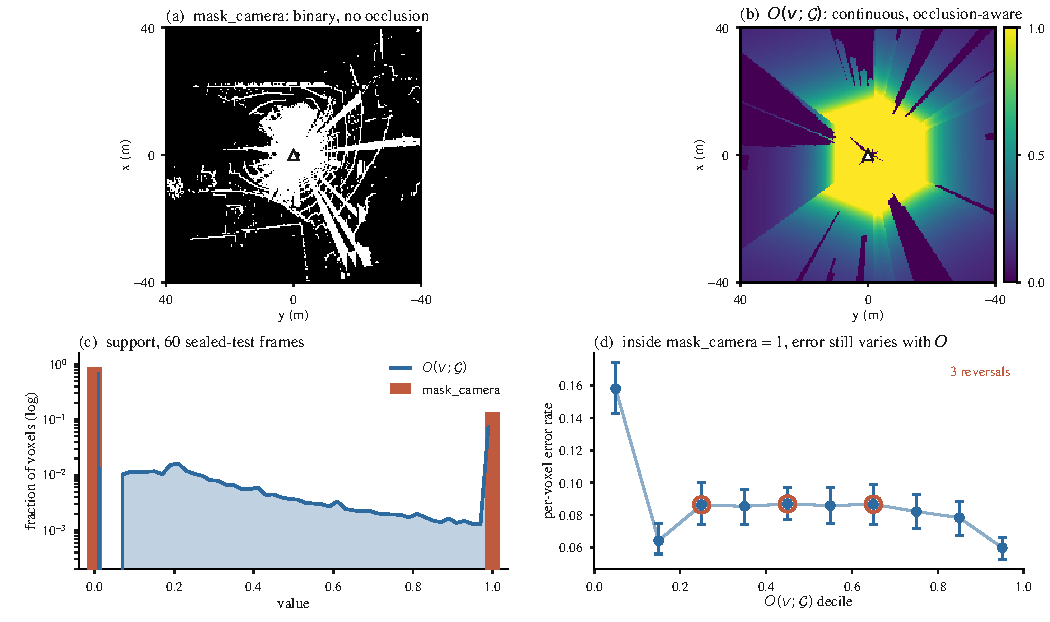
\includegraphics[width=\textwidth]{fig3_whynotmask.pdf}
\caption{\textbf{Why not \texttt{mask\_camera}, argued on the data.}
All four panels are the same frame. \texttt{mask\_camera} is the obvious
objection to this paper and it does not survive contact with its own
definition: it is binary, it is constructed offline from the full sensor
suite including the LiDAR the model never receives, and it is not available
at inference, so inside the mask it is constant and ranks nothing. Range
from ego is continuous and free, and ignores occlusion, which is the entire
phenomenon. Observability is continuous, camera-only, known before the
network runs, and resolves occlusion by first-hit ray marching.}
\label{fig:maskcam}
\end{figure*}

% -------------------------------------------------------------------
\section{Experiments}

\subsection{Setup}
\paragraph{Model and data.}
FB-OCC r50 with temporal fusion on Occ3D-nuScenes, $200\times200\times16$
voxels at 0.4\,m, 18 classes. We measure mIoU $38.90$ against a
published $39.1$, so the checkpoint reproduces.

\paragraph{The sealed split.}
The 150 validation scenes are partitioned once into a development half and
a held-out test half of \nScenes\ scenes, recorded under digest
\splitdigest. Method development used the development half only; the test
half was opened once. A single module is the source of truth for the
split, and every script and every CI gate reads it from there.

\paragraph{Statistics.}
AUROC by exact histogram on quantised scores; paired scene bootstrap for
all intervals; risk-coverage and AURC for selective prediction; ECE in 15
bins.

\subsection{Observability outranks the camera mask}
\label{sec:h2}
Scoring per-voxel error inside \texttt{mask\_camera}, where the mask is
constant and therefore ranks nothing, observability reaches an AUROC of
$0.6321$. The pre-registered contrast H2 against the mask is
\Hii\ \HiiCI\ on the test half, and $+0.0534$ on the full 150 scenes; the
test figure is the one we quote, and the two are given together so the
difference cannot be mistaken for a selection effect.

This is a modest effect in absolute terms and we do not inflate it. Its
interest is that it is obtained by a quantity that costs no training, reads
nothing from the network, and is available before the forward pass.

\subsection{The granularity inversion}
At the voxel level, maximum softmax probability reaches \voxMSP\ against
observability's \voxObs. At the frame level the ordering holds but
narrows, \frmConf\ against \frmObs. At the object level it reverses:
observability reaches \objObs\ against confidence's \objMSP, a gain of
\objDelta\ \objDeltaCI\ over \nObj\ objects in \nFrames\ frames.

A LiDAR point-count oracle, which sees the modality the model does not,
reaches \objOracle. Observability is within noise of it.

% generated by scripts/paper/table1_perclass.py -- do not edit
\definecolor{odfmshade}{gray}{0.93}
\definecolor{swcar}{HTML}{3182BD}
\definecolor{swtruck}{HTML}{D62728}
\definecolor{swbus}{HTML}{FFD700}
\definecolor{swtrailer}{HTML}{8B4513}
\definecolor{swconstructionvehicle}{HTML}{40E0D0}
\definecolor{swpedestrian}{HTML}{FF0000}
\definecolor{swmotorcycle}{HTML}{808000}
\definecolor{swbicycle}{HTML}{FFC0CB}
\begin{table}[t]\centering\footnotesize
\setlength{\tabcolsep}{2.05pt}
\caption{\textbf{Per class, object level, sealed test split.} \emph{missed} is the fraction of annotated objects the model never predicts. AUROC columns rank that event. \textsc{oracle} counts LiDAR returns inside the box and therefore sees a modality the model does not; it is an upper reference, not a competitor. Observability wins on the two largest classes and loses on trailer and bicycle, and both losses are printed.}
\label{tab:perclass}
\begin{tabular}{llrrccc>{\columncolor{odfmshade}}c}
\toprule
& Class & $n$ & missed & \multicolumn{3}{c}{AUROC $\uparrow$} & obs$-$conf \\
\cmidrule(lr){5-7}
& & & & conf. & obs. & \textsc{orac.} & $\Delta$ \\
\midrule
\textcolor{swcar}{$\blacksquare$} & car & 22,096 & 11.8\% & 0.681 & \textbf{0.832} & 0.786 & \textbf{+0.152} \\
\textcolor{swpedestrian}{$\blacksquare$} & pedestrian & 10,407 & 36.2\% & \textbf{0.711} & 0.707 & 0.739 & -0.004 \\
\textcolor{swtruck}{$\blacksquare$} & truck & 3,956 & 11.6\% & 0.696 & \textbf{0.786} & 0.765 & \textbf{+0.089} \\
\textcolor{swtrailer}{$\blacksquare$} & trailer & 1,056 & 11.5\% & \textbf{0.776} & 0.553 & 0.630 & -0.198 \\
\textcolor{swmotorcycle}{$\blacksquare$} & motorcycle & 1,011 & 25.4\% & 0.673 & \textbf{0.720} & 0.714 & +0.047 \\
\textcolor{swbicycle}{$\blacksquare$} & bicycle & 982 & 33.2\% & \textbf{0.820} & 0.708 & 0.723 & \textbf{-0.115} \\
\textcolor{swbus}{$\blacksquare$} & bus & 814 & 13.3\% & \textbf{0.731} & 0.723 & 0.744 & -0.001 \\
\textcolor{swconstructionvehicle}{$\blacksquare$} & construction vehicle & 541 & 48.2\% & \textbf{0.729} & 0.646 & 0.656 & -0.087 \\
\midrule
& \textbf{all dynamic} & 40,863 & 19.3\% & 0.719 & \textbf{0.762} & 0.774 & \textbf{+0.043} \\
\bottomrule
\end{tabular}
\end{table}


\Cref{tab:perclass} breaks this down. Observability wins decisively on
car, the largest class by a factor of two ($+0.152$), and on truck
($+0.089$). It loses on trailer ($-0.198$) and bicycle ($-0.115$), and
ties on the rest. Both losses are consistent with the mechanism rather
than against it: a trailer is large enough that some part of it is almost
always observed, so observability is near-constant across the class and
has little left to rank, while the model's confidence still varies.

\subsection{Downstream: selective prediction}
A ranking score is only useful if abstaining on its worst-ranked fraction
actually lowers risk. Measuring area under the risk-coverage curve
(AURC, lower is better) on the sensor-only volume:
\begin{center}\small
\begin{tabular}{lc}
\toprule
Score & AURC $\downarrow$ \\
\midrule
confidence alone                & 0.2526 \\
confidence + \texttt{mask\_camera} & \textbf{0.2128} \\
confidence + observability      & 0.2160 \\
observability alone             & 0.3156 \\
\texttt{mask\_camera} alone     & 0.3542 \\
\bottomrule
\end{tabular}
\end{center}
Adding observability to confidence reduces AURC by
$0.0365$ $[0.0307, 0.0425]$, which holds. Against
confidence plus \texttt{mask\_camera} it is $-0.0033$
$[-0.0051, -0.0015]$: \textbf{observability loses this comparison, and the
interval excludes zero.} We report it because an oracle mask built from the
full sensor suite offline ought to win a volume-level abstention test, and
because the object-level result in \cref{tab:perclass} is not weakened by
it. The two measure different things, and only one of them is available on
a vehicle.

\subsection{Ablations}
\label{sec:ablations}
\paragraph{Temporal accumulation.} Propagating past observability through
ego poses with an exponential half-life, and scoring on the same voxels:
half-lives of $0.5$, $1$, $2$ and $4$\,s give $+0.0080$, $+0.0083$,
$+0.0156$ and $+0.0196$ AUROC over the instantaneous map. The half-life was
fixed at $2$\,s before the run; at that value the interval is
$[+0.0098, +0.0214]$ and H4 holds. The monotone trend to $4$\,s is reported
but was not registered and is not claimed.

\paragraph{Temperature scaling is not a competitor.} It is a monotone
transform of the confidence score, so it leaves every ranking metric in this
paper exactly unchanged. It appears in no AUROC table here, and a reviewer
should expect its absence.

\paragraph{Which term carries the result.} \Cref{eq:obs} has two factors and
a pooling choice, and only one of the three matters. Scoring per-voxel error
on 675 frames across 145 scenes:
\begin{center}\small
\begin{tabular}{lcc}
\toprule
Variant & AUROC $\uparrow$ & vs \texttt{mask\_camera} \\
\midrule
$\max_i c_i s_i$ \;(ours)        & \textbf{0.6755} & $+0.0575$ \\
sum over cameras                 & 0.6748 & $+0.0568$ \\
no temporal term                 & 0.6755 & $+0.0575$ \\
\textbf{no visibility term} $s_i$ & 0.5908 & $\mathbf{-0.0272}$ \\
\texttt{mask\_camera}            & 0.6180 & --- \\
\bottomrule
\end{tabular}
\end{center}
Pooling by maximum rather than by sum is worth $+0.0007$, which is nothing;
we keep the maximum because it is the one with a reading ("seen well by at
least one camera"), not because it measures better. Dropping the visibility
factor, so that coverage alone decides, costs $0.0847$ AUROC and drops the
score \emph{below} \texttt{mask\_camera}. Resolving occlusion is not a
refinement of this measure. It is the measure.

\paragraph{Would a seventh camera fix it?} On 1{,}238 frames, $76.6\%$ of
ground-truth obstacle voxels fall in volumes with no camera evidence. We
re-ran the geometry with each of six additional camera placements added to
the rig. The best of them, a higher roof mount, recovers $2.23\%$ of those
voxels; a rear telephoto recovers $1.29\%$; no other placement exceeds
$0.8\%$. The blind volume is not an artifact of this particular rig and is
not closed by adding a sensor to it, which is the argument for measuring it
rather than engineering it away.

\subsection{What did not survive}
% generated by scripts/paper/table4_ledger.py -- do not edit by hand
\begin{table*}[t]
\centering\footnotesize\setlength{\tabcolsep}{4pt}
\caption{\textbf{All measured contrasts.} Paired scene-bootstrap means with 95\% intervals on the sealed test split (75 scenes, 3,008 frames); AUROC difference unless noted. Each contrast was specified before its data existed, and every one that was specified is listed here.}
\label{tab:ledger}
\begin{tabular}{@{}ll r@{}}
\toprule
 & Contrast & $\Delta$AUROC [95\% CI] \\
\midrule
\multicolumn{3}{@{}l}{\emph{Per voxel}} \\
H2 & Observability vs.\ \texttt{mask\_camera} & +0.0484 [+0.0390, +0.0584] \\
H4 & Temporal vs.\ instantaneous observability & +0.0156 [+0.0098, +0.0214] \\
H5 & Combined score vs.\ observability alone & +0.2491 [+0.2407, +0.2575] \\
H6 & Combined score vs.\ model confidence & +0.0015 [+0.0009, +0.0022] \\
H1 & Calibration gap vs.\ observability decile & $\rho = -0.433$, 2 reversals \\
\midrule
\multicolumn{3}{@{}l}{\emph{Per object}} \\
E1 & Observability vs.\ model confidence & +0.0432 [+0.0135, +0.0708] \\
E2 & Observability vs.\ LiDAR point-count oracle & -0.0121 [-0.0289, +0.0052] \\
A55 & Predicted-geometry occluder vs.\ model confidence & -0.0477 [-0.0828, -0.0135] \\
\midrule
\multicolumn{3}{@{}l}{\emph{Selective prediction and calibration}} \\
S1 & Observability vs.\ confidence, selective risk & +0.0365 [+0.0307, +0.0425] \\
S2 & Observability vs.\ \texttt{mask\_camera}, selective risk & -0.0033 [-0.0051, -0.0015] \\
R1 & Observability-conditioned vs.\ global recalibration, ECE & +0.0026 [-0.0026, +0.0058] \\
\bottomrule
\end{tabular}
\end{table*}


% TODO(pod): H2' on SurroundOcc. Registered in METHOD_FREEZE A53 with
% acceptance >= +0.02 and an interval excluding zero, before the run.
% TODO(pod): MC-dropout and deep-ensemble rows. Currently the single
% largest gap in the evaluation.

% -------------------------------------------------------------------
\section{Conclusion}
Observability is a geometric quantity with one parameter and no learned
component, and it predicts where a camera-only occupancy model is about to
fail. Its value is not uniform across granularity, and that non-uniformity
is the result: the model's own confidence is the better signal for whether a
voxel is wrong, and the worse signal for whether an object is missing
entirely, because a missed object is a confident prediction of free space.
Geometry has no such blind spot, since it never consults the model. We
report four failed hypotheses alongside the successful ones and a selective
prediction comparison that observability loses, because an evaluation
protocol that only produces agreeable results is not measuring anything.

{\small
\bibliographystyle{ieeetr}
\bibliography{../opendrivefm_refs}
}

\end{document}
